\documentclass{article}
\usepackage{graphicx}
\usepackage{polski}
\usepackage{hyperref}
\usepackage{amssymb}
\title{Podstawy sztucznej inteligencji - sprawozdanie}
\author{Dawid Kania}
\date{February 2025}

\begin{document}
	\maketitle
	\newpage
	\section{Wstęp}
	Kod źródłowy znajduje się pod linkiem:
	\url{https://github.com/Kaniek99/AIbasics}\\ Wszystkie problemy zostały rozwiązane
	zgodnie z algorytmem omawianym na zajęciach -- tzn. generujemy jednego rodzica
	a następnie przez mutację tworzymy dziecko. Zastosowanie dla poszczególnych
	problemów zostanie omówione szczegółowo w rozdziałach poświęconych danym
	problemom. Rozwiązanie każdego problemu znajduje się w oddzielnym pliku, część
	wspólna znajduje się w pliku
	\href{https://github.com/Kaniek99/AIbasics/blob/main/src/genotype/genotype.go}{genotype.go}
	i zawiera interfejs $Genotype$ z metodami $Mutate,\ Swap,\ Crossover$.
	\section{Problem plecakowy}
	Problem plecakowy to problem optymalizacyjny, w którym maksymalizujemy wartość
	przedmiotów spakowanych do plecaka. Przedmioty mają swoją wagę/objętość a liczba
	spakowanych rzeczy jest ograniczona przez pojemność plecaka.
	\subsection{Założenia}
	Niech $I$ będzie zbiorem przedmiotów, wówczas $i_{i}$ jest $i$-tym przedmiotem
	z tego zbioru. Przez $w_{i}$ oznaczamy wagę $i$-tego przedmiotu a przez
	$v_{i}$ jego wartość. Rozwiązaniem jest ciag binarny $s$ o liczebności równej liczebności
	zbioru przedmiotów. Maksymalną dopuszczalną wagę plecaka oznaczamy przez
	$w_{max}$ natomiast wyrażenie $i_{i}\in P$ oznacza, że $i$-ty przedmiot należy
	do ciągu binarnego plecaka P. Wówczas dane wejściowe to:
	\begin{itemize}
		\item $|I| = |s| = 100$,

		\item $v_{i}\in[10,90]\ \wedge\ v_{i}\in\mathbb{N}$,

		\item $w_{i}\in[10,90]\ \wedge\ w_{i}\in\mathbb{N}$,

		\item $w_{max}= 2500$,

		\item $s_{i}=\left\{
			\begin{array}{l}
				1,\ i_i\in P,     \\
				0,\ i_i\not\in P.
			\end{array}\right.$
	\end{itemize}
	\subsection{Rozwiązanie problemu}
	Niech $s$ będzie ciągiem binarnym będącym rozwiązaniem problemu, wówczas
	współczynnik dopasowania dla $s$ wyznaczamy według następującej formuły:
	\[
		f(s) = \left\{
		\begin{array}{l}
			\sum_{i\in P}v_i,\ gdy\ \sum_{i\in P}w_i < w_{max},    \\
			w_{max} - \sum_{i\in P}w_i,\ w\ przeciwnym\ przypadku.
		\end{array}\right.
	\]
	\textbf{Algorytm genetyczny służący do rozwiązania problemu plecakowego}\\ Warunkiem
	kończącym działanie algorytmu jest nieznalezienie lepszego rozwiązania przez 100
	iteracji.\\ Krok 1. Wygenerowanie zbioru przedmiotów $I$\\ Krok 2.
	Wygenerowanie rodzica $s$\\ Krok 3. Obliczamy $f(s)$.\\ Krok 4. Sprawdzamy czy
	licznik iteracji zakończonych niepowodzeniem jest mniejszy niż 100. Jeśli nie to
	algorytm kończy działanie.\\ Krok 5. Dziecko $c$ powstaje przez mutację rodzica
	-- losowo wybrany gen zmienia wartość na przeciwną.\\ Krok 6. Obliczamy $f(c)$.\\
	Krok 7. Rozważamy teraz dwa przypadki:
	\begin{itemize}
		\item $f(s)<f(c)$ Zatem lepszym rozwiązaniem jest dziecko -- staje się ono
			teraz rodzicem, $s=c, f(s)=f(c)$. Licznik iteracji zakończonych
			niepowodzeniem ustawiamy na 0. Wracamy do kroku 4.

		\item $f(s)\geq f(c)$\\ Zwiększamy licznik iteracji zakończonych
			niepowodzeniem. Wracamy do kroku 4.
	\end{itemize}
	Na wyjściu otrzymujemy rozwiązanie suboptymalne.\\ Implementacja rozwiązania powyższego
	problemu znajduje się w pliku \href{https://github.com/Kaniek99/AIbasics/blob/main/src/knapsack/knapsack.go}{knapsack.go}\\
	\textbf{Przykładowe rozwiązanie}\\
	\begin{figure}[h]
		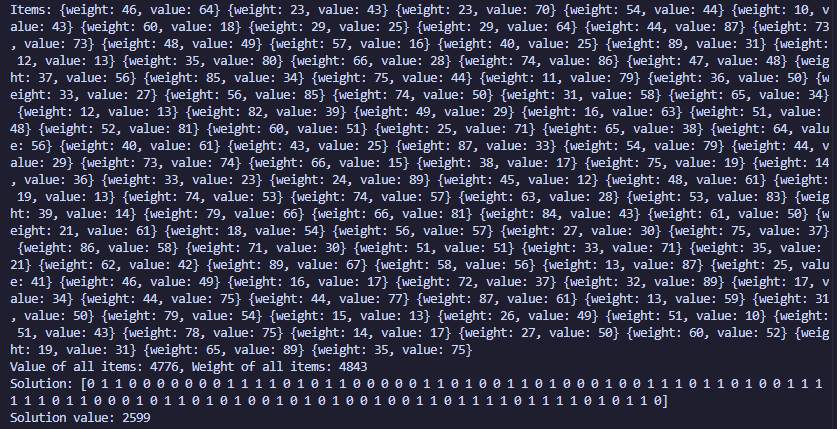
\includegraphics[width=\linewidth]{knapsack_example.png}
	\end{figure}
	\newpage
	\section{Problem alokacji zadań}
	Problem alokacji zadań to problem optymalizacyjny, w którym należy przydzielić
	wszystkie zadania na dostępne rdzenie procesora w taki sposób aby łączny czas ich
	wykonania był jak najkrótszy. Każdy z rdzeni ma pewien mnożnik, z którym wykonuje
	zadania.
	\subsection{Założenia}
	Niech $T$ będzie zbiorem zadań, wówczas $t:T\rightarrow \mathbb{Z_+}$ jest ciągiem,
	który $i-temu$ zadaniu przypisuje czas $t_{i}$ potrzebny do jego wykonania. Zbiór
	$C$ jest zbiorem ID rdzeni procesora gdzie $c_{i}$ to ID $i$-tego rdzenia a $C_{i}$
	to zbiór zadań wykonywanych na $i$-tym rdzeniu. Rozwiązaniem jest ciag
	$s:T\rightarrow C$, o liczebności równej liczebności zbioru zadań, którego
	elementami są liczby całkowite. Ciąg z mnożnikami rdzeni oznaczamy przez $m$,
	jego liczebność jest równa zbiorowi rdzeni a $i$-ty element ciągu to mnożnik
	$i$-tego procesora. Wówczas dane wejściowe to:
	\begin{itemize}
		\item $|T|=|s|=100$

		\item $|C|=|m|=4$

		\item $i\in\{0,\ 1,\ 2,\ ...\ ,\ 99\}$

		\item $c_{i}\in\{0,\ 1,\ 2,\ 3\}$

		\item $s_{i}\in C$

		\item $m=(1,\ 1.25,\ 1.5,\ 1.75)$

		\item $|s|=|T|=100$
	\end{itemize}
	\subsection{Rozwiązanie problemu}
	Niech $s$ będzie rozwiązaniem problemu, wówczas współczynnik dopasowania dla $s$
	wyznaczamy według następującej formuły:
	\[
		f(s)=max(\sum_{i\in C_0}t_{i}m_{0},\sum_{i\in C_1}t_{i}m_{1},\ ...\ ,\sum_{i\in
		C_3}t_{i}m_{3})
	\]
	\textbf{Algorytm genetyczny służący do rozwiązania problemu alokacji zadań}\\
	Warunkiem kończącym działanie algorytmu jest nieznalezienie lepszego
	rozwiązania przez 100 iteracji.\\ Krok 1. Wygenerowanie zbioru zadań $T$ oraz
	funkcji $t:T\rightarrow \mathbb{Z_+}$\\ Krok 2. Wygenerowanie rodzica $s$\\
	Krok 3. Obliczamy $f(s)$.\\ Krok 4. Sprawdzamy czy licznik iteracji
	zakończonych niepowodzeniem jest mniejszy niż 100. Jeśli nie to algorytm
	kończy działanie.\\ Krok 5. Dziecko $d$ powstaje przez mutację rodzica -- losowo
	wybrany gen zmienia wartość -- odpowiada to przypisaniu zadania do innego
	rdzenia.\\ Krok 6. Obliczamy $f(d)$.\\ Krok 7. Rozważamy teraz dwa przypadki:
	\begin{itemize}
		\item $f(s) < f(d)$ Zwiększamy licznik iteracji zakończonych niepowodzeniem.
			Wracamy do kroku 4.

		\item $f(s)\geq f(d)$\\ Zatem lepszym rozwiązaniem jest dziecko -- staje się
			ono teraz rodzicem, $s=d, f(s)=f(d)$. Licznik iteracji zakończonych niepowodzeniem
			ustawiamy na 0. Wracamy do kroku 4.
	\end{itemize}
	Na wyjściu otrzymujemy rozwiązanie suboptymalne.\\ Implementacja rozwiązania powyższego
	problemu znajduje się w pliku \href{https://github.com/Kaniek99/AIbasics/blob/main/src/allocation/allocation.go}{allocation.go}\\
	\textbf{Przykładowe rozwiązanie}\\
	\begin{figure}[h]
		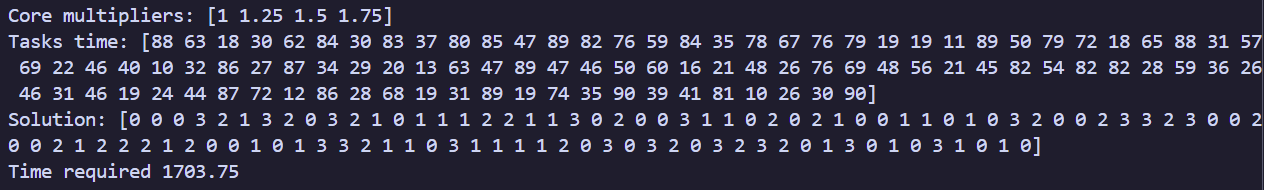
\includegraphics[width=\linewidth]{allocation_example.png}
	\end{figure}
	\newpage
	\section{Problem komiwojażera}
	Problem komiwojażera to problem optymalizacyjny, w którym należy wyznaczyć jak
	najkrótszą trasę prowadzącą przez wszystkie miasta.
	\subsection{Założenia}
	Niech $C$ będzie zbiorem identyfikatorów miast, wówczas $d:C\times C\rightarrow
	\mathbb{R_+}$ jest funkcją, która parze miast $(c_{i},c_{j})$ przypisuje
	odległość $d_{ij}$ pomiędzy nimi. Rozwiązaniem problemu nazywamy dowolną permutację
	zbioru $C$ i oznaczamy ją przez $s$. Wówczas dane wejściowe to:
	\begin{itemize}
		\item $C=\{0,\ 1,\ 2,\ ...\ ,\ 99\}$

		\item $s:C\rightarrow C$

		\item $\left\{
			\begin{array}{l}
				d(i,j) = d(j,i),      \\
				d(i,j) > 0,\ i\neq j, \\
				d(i,j)=0,\ i=j.
			\end{array}\right.$
	\end{itemize}
	\subsection{Rozwiązanie problemu}
	Niech $s$ będzie rozwiązaniem problemu, wówczas współczynnik dopasowania dla
	$s$ wyznaczamy według następującej formuły:
	\[
		f(s)=\sum_{i=1}^{|C|-1}d(s_{i-1},s_{i})
	\]
	\textbf{Algorytm genetyczny służący do rozwiązania problemu alokacji zadań}\\ Warunkiem
	kończącym działanie algorytmu jest nieznalezienie lepszego rozwiązania przez 100
	iteracji.\\ Krok 1. Wygenerowanie odległości pomiędzy miastami --
	$d:C\times C\rightarrow \mathbb{R_+}$\\ Krok 2. Wygenerowanie rodzica $s$\\
	Krok 3. Obliczamy $f(s)$.\\ Krok 4. Sprawdzamy czy licznik iteracji
	zakończonych niepowodzeniem jest mniejszy niż 100. Jeśli nie to algorytm
	kończy działanie.\\ Krok 5. Dziecko $k$ powstaje przez zamienienie miejscami
	dwóch losowo wybranych genów u rodzica.\\ Krok 6. Obliczamy $f(k)$.\\ Krok 7.
	Rozważamy teraz dwa przypadki:
	\begin{itemize}
		\item $f(s) < f(k)$ Zwiększamy licznik iteracji zakończonych niepowodzeniem.
			Wracamy do kroku 4.

		\item $f(s)\geq f(k)$\\ Zatem lepszym rozwiązaniem jest dziecko -- staje się
			ono teraz rodzicem, $s=k, f(s)=f(k)$. Licznik iteracji zakończonych niepowodzeniem
			ustawiamy na 0. Wracamy do kroku 4.
	\end{itemize}
	Na wyjściu otrzymujemy rozwiązanie suboptymalne.\\ Implementacja rozwiązania powyższego
	problemu znajduje się w pliku \href{https://github.com/Kaniek99/AIbasics/blob/main/src/salesman/salesman.go}{salesman.go}\\
	\textbf{Przykładowe rozwiązanie}\\
	\begin{figure}[h]
		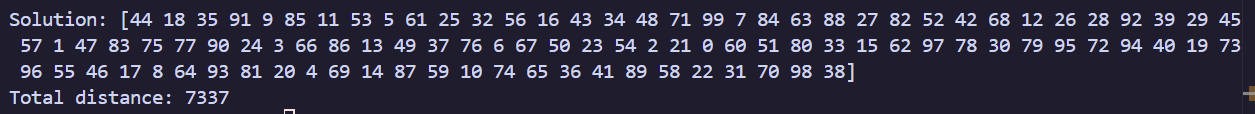
\includegraphics[width=\linewidth]{salesman_example.png}
	\end{figure}
\end{document}